\documentclass{school-22.101-notes}
\date{November 9, 2011}

\begin{document}
\maketitle


\topic{Ground-state Spin-Parity Assignments/Predictions}
Notation: \ce{^A_p X_n}, proton number determines the type of isotope, neutron number determines isotones.  

We define a \textbf{Total Angular Momentum of Nucleus} to be $I$, and define parity to be $\pi = (-1)^l$. We are going to use the right-hand of Figure~\ref{ns-magic-numbers}.
\begin{figure}[ht]
    \centering
    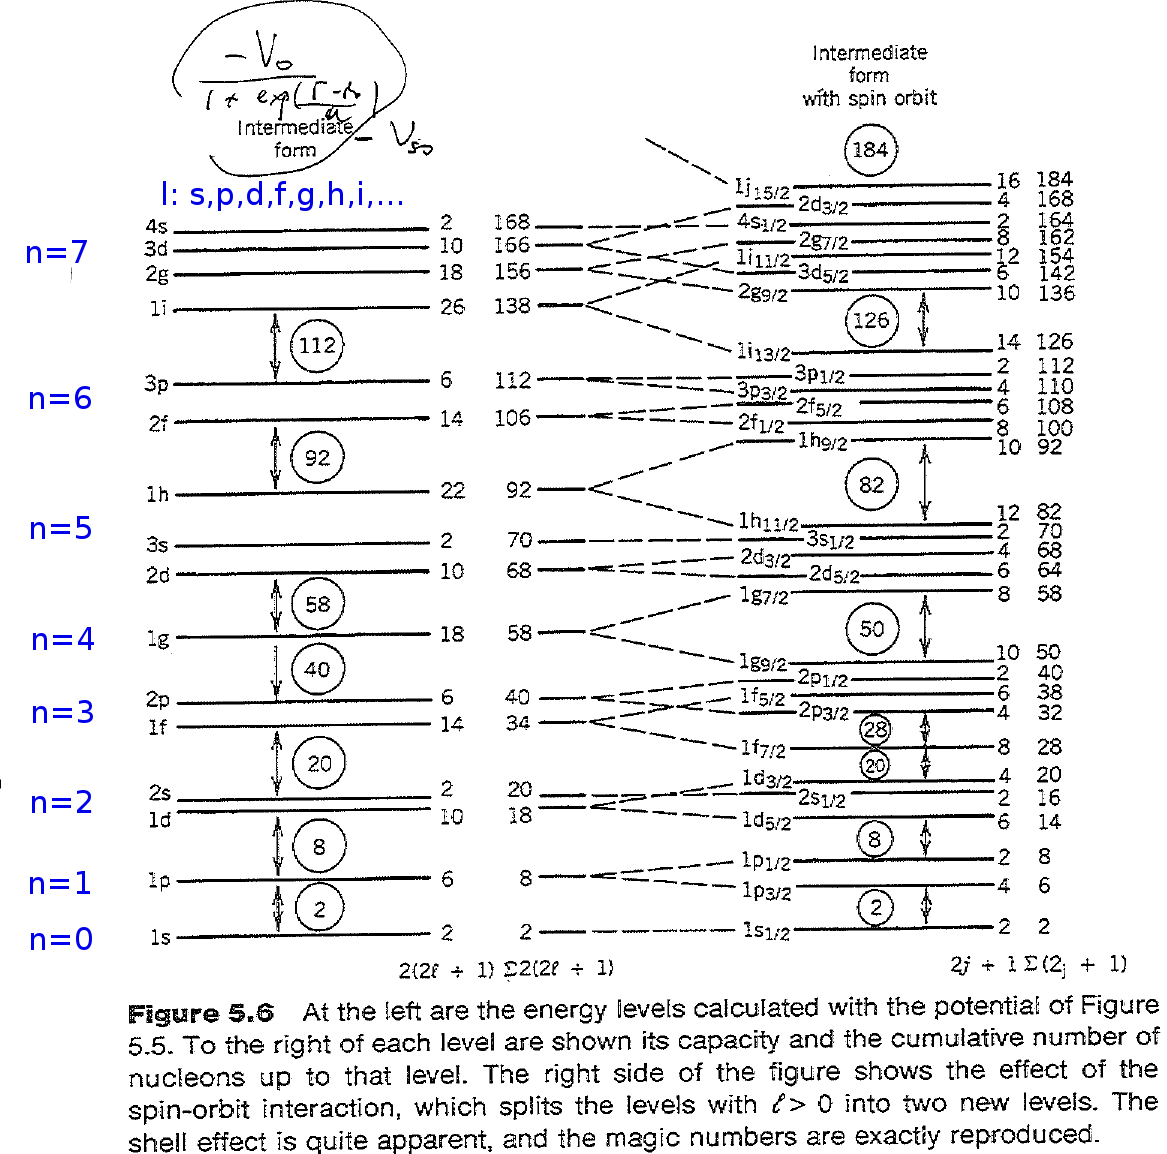
\includegraphics[width=5in]{images/ns/magic-numbers.png}
    \caption{Energy Occupation Diagram}
    \label{ns-magic-numbers}
\end{figure}

\clearpage
\subtopic{Nuclei with Odd A (\# of neutrons plus protons)} 
Example: compare \ce{^{15}_{8}O_7} and \ce{^{17}_8 O_9} in Fig.~\ref{odd-A-nuclide}, we notice that the last nucleon filling the shell model is the one that contributes to the structure. 

\begin{figure}[ht]
  \centering
  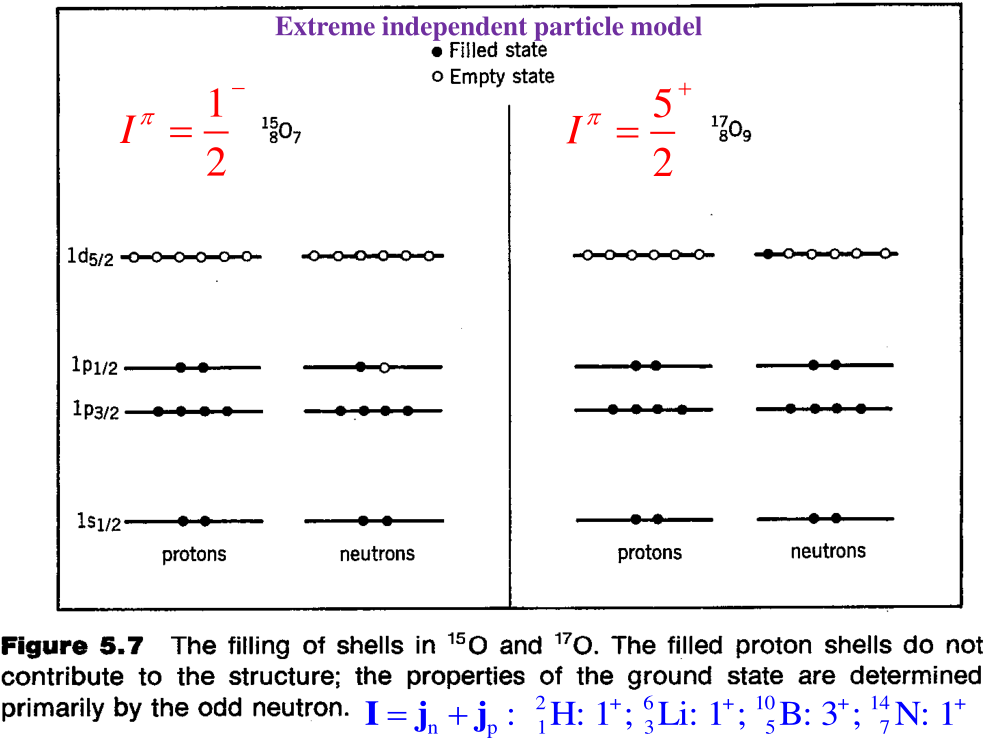
\includegraphics[width=4.5in]{images/ns/odd-A-nuclide.png}
  \caption{The Last Nucleon Contributes To the Structure} \label{odd-A-nuclide}
\end{figure}

Process: 
\begin{enumerate}
\item Determine the number of neutrons, protons from \ce{^A_p X_n};
\item For protons or neutrons whichever is odd, fill in the shell models; do so by start from the bottom level, each level hosts $2j+1$ number of protons; the highest level determines the $l$ value we use to fine $\pi$, and the $j$ value associated with this level is the $I$ term;
\item For now we don't care about the even number nucleons. 
\end{enumerate}

\textbf{Pairing Effect for Larger $l$}: the residual terms we ignored at calculating single-particle Hamiltonian have an effect at short range for nucleons, resulting in a decreased energy and the orbital angular momentum tends to claps to zero. So the state with larger $l$ value is more favored to be filled. 

Example: \ce{^{207}_{82} Pb_{125}}, see Figure~\ref{ns-Pb-125}.
\begin{figure}[ht]
    \centering
    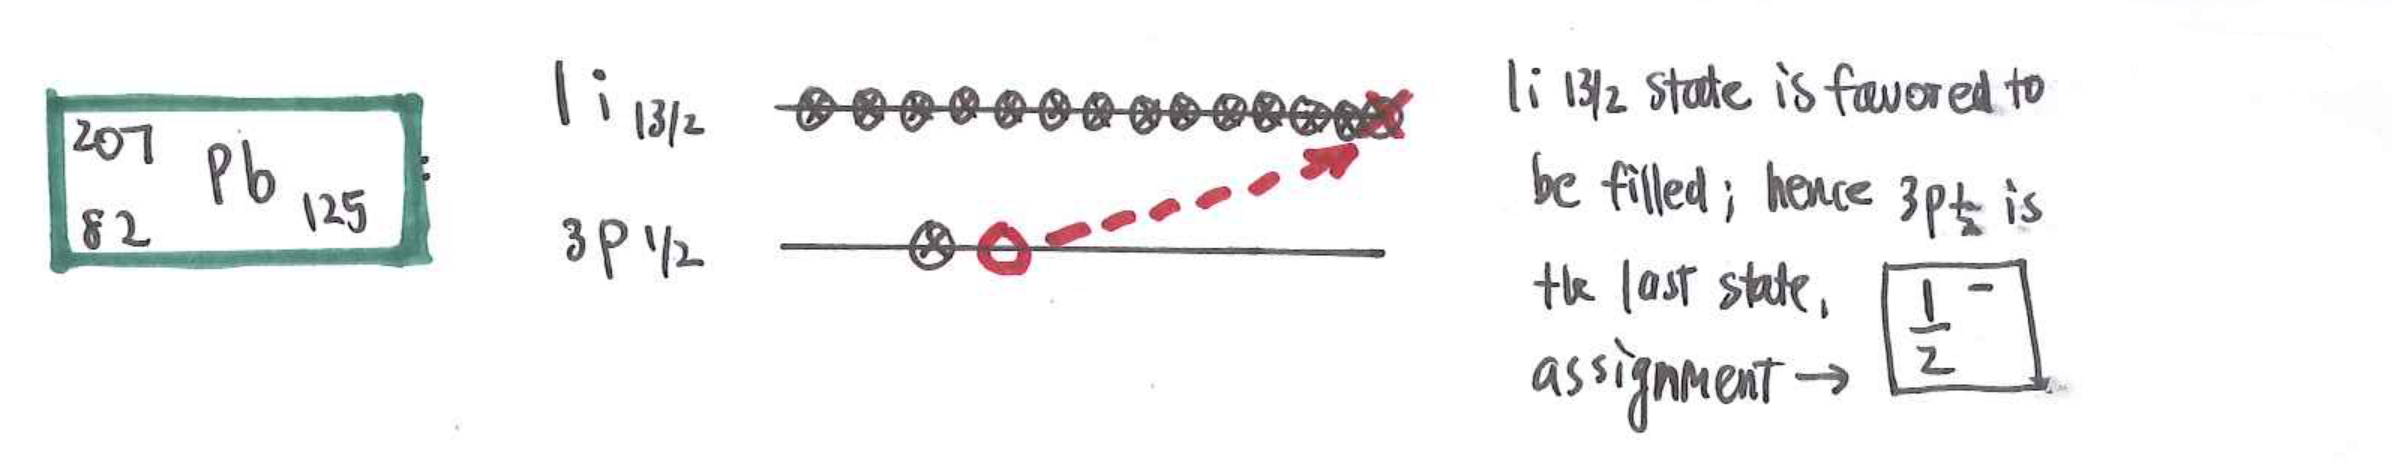
\includegraphics[width=5in]{images/ns/Pb-125.png}
    \caption{Paring Effect Illustration (Odd A): Pb-125}
    \label{ns-Pb-125}
\end{figure}



\subtopic{Even Neutron, Even Proton} 
Derived from the paring effect, nucleons want to minimize the energy by setting the pair's angular momentum to zero. Among the hundreds of stable or radioactive even-Z even-N nuclides, all have $I=0$. This is strong evidence for the nuclear paring force. Example: \ce{^{40}_{20}Ca_{20}}, \ce{^{36}_{18} A_{18}}, \ce{^{130}_{36} Sn_{80}}, $\cdots$. 


\subtopic{Odd Neutron, Odd Proton}
There are only 4 stable odd-Z odd-N nuclides: \ce{_1 H_1}, \ce{_3 Li_3}, \ce{_5 B_5}, \ce{_7 N_7}. 


There is a tendency to align the spin of the last neutron state and the last proton state. We can flip either state, as long as we take the magnitude of the resulting $I$. See approach one of \ce{^{38} Cl_{21}} in Figure~\ref{ns-Cl-21}.
\begin{figure}[ht]
    \centering
    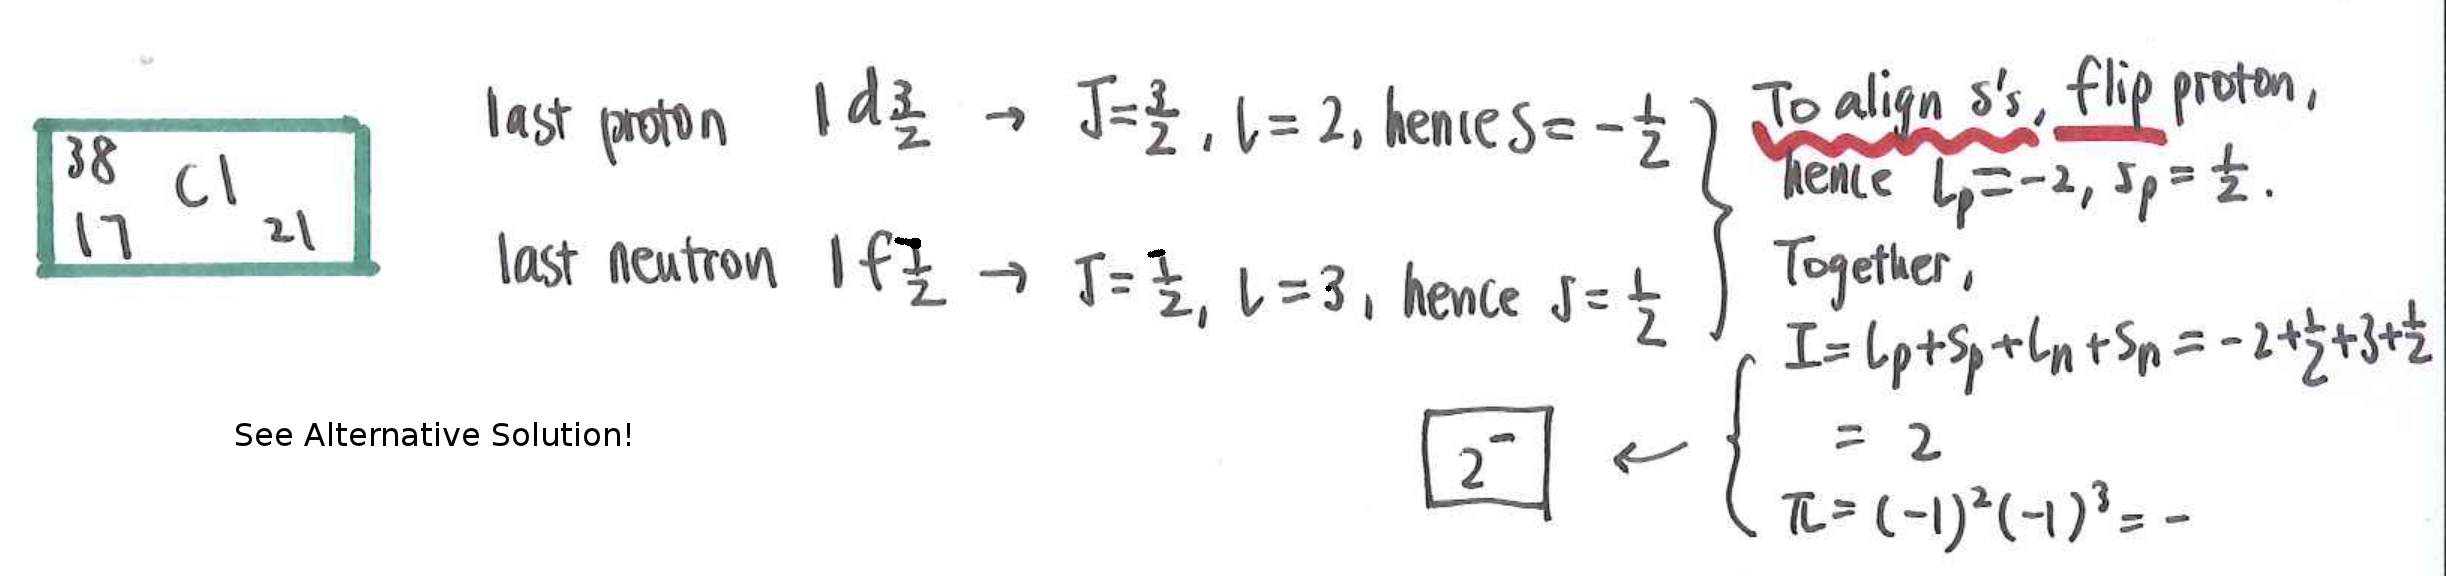
\includegraphics[width=5in]{images/ns/Cl-21.png}
    \caption{Flip Spin Effect Illustration (Odd-Odd): Cl-21}
    \label{ns-Cl-21}
\end{figure}

Alternative approach: Again we look at the last neutron and last proton, which are $1d_{3/2}, 1f_{7/2}$. Immediately we know $ \frac{7}{2} - \frac{3}{2} \le I \le \frac{7}{2} + \frac{3}{2}$. Consider Table~\ref{spin-l}, we know one is spin up, one is spin down, that is suggesting, we pick the opposite case for $I$, that is, $I=\frac{7}{2} - \frac{3}{2} =2$. The spin part is $(-1)^{L_p} (-1)^{L_n} = (-1)^3 (-1)^2 = -1$. Hence the result is $2^-$.  
\begin{table}[ht]
\centering
\begin{tabular}{|c|c|c|} \hline
l & spectro & Spin \\ \hline
0 & s & + \\ \hline
1 & p & - \\ \hline
2 & d & + \\ \hline
3 & f & - \\ \hline
4 & g & + \\ \hline
\end{tabular}
\caption{Spin Based on $l$\label{spin-l}}
\end{table}

%%%%%%%%%%%%%%%%%%%%%%%%% Part 3: Radioactive Decay %%%%%%%%%%%%%%%%
\lecture{Radioactive Decay}
We have been talking about the stable cases only (nuclear binding). Now we are going to move to the unstable cases (transition), including spontaneous decays, and nuclear reactions (induce/bombard). This discussion would relate nuclear binding energy to nuclear mass. 

\ce{^1H ->[+n] ^2_1H_1 ->[+n] ^3H} (stable)  \ce{->[\beta] ^3He} (unstable) \ce{ ->[+n] ^4He} (very stable, because double magic 2n + 2p). 

\ce{^4He} can get a neutron to become \ce{^5He}, but the half life is very short ($3 \times 10^{-21}$ s); similarly if \ce{^4He} gets a proton to form \ce{^5Li} its half-life is on the order of $10^{-22} \s$. It appears that it is impossible to make heavy nuclei, which is of course not the case. This leads us to the inter-connection between nuclei mass, binding energy, and energy released or absorbed in nuclear reactions.

\topic{Binding Energy}
Binding energy of a nucleus with A,Z is:
\begin{align} 
B(A,Z) &= \left[ Z m_p + N m_n - (m(A,Z) - Z m_e) \right] c^2 \\
&= \left[ Z m_{\ce{^1 H}} + N m_n - m(A,Z) \right] c^2
\end{align}
Binding energy for the outmost neutron (`valence' nucleon) $=$ neutron separation energy $=$ the energy required to separate one neutron from a nucleus; similarly for proton separation energy: 
\begin{align}
S_n &= B(\ce{^A_Z X_N}) -B(\ce{^{A-1}_Z X_{N-1}}) = \left[ m(A-1, Z) - m(A,Z) + m_n \right] c^2 \\
S_p &= B(\ce{^A_Z X_N}) -B(\ce{^{A-1}_{Z-1} X_{N}}) = \left[ m(A-1, Z-1) - m(A,Z) + m_{H} \right] c^2
\end{align}

\subtopic{Binding Energy as a Function of A}
\begin{enumerate}
\item As A increases, Total Binding Energy increases; 
\item BE per nucleon, B/A, is not a linear relationship with A.
    \begin{enumerate}
    \item For small A up to $A = 60$ (\ce{^{56} Fe}, \ce{^{58} Fe}, \ce{^{62} Ni}), B/A, hence the isotopes become more stable; hence fusion is applicable in this region because we gain energy as we bring small A particles together; 
    \item Beyond $A = 60$, as A increases, B/A decreases very gradually, relatively constant for most nuclei with B/A around 8 MeV. Fission is applicable in this case because we can gain energy by splitting/decreasing A. 
    \end{enumerate}  
\end{enumerate}




\end{document}
